%META {"question":"Tia Ox và tia OM chung gốc O, cùng đi qua điểm M. Hai tia này là hai tia gì?","options":["Trùng nhau","Đối nhau","Không chung gốc","Vuông góc với nhau"],"answer":0,"note":"Hai tia chung gốc và cùng hướng (cùng đi qua điểm M) thì trùng nhau."}
\documentclass[border=5pt]{standalone}
\usepackage{tkz-euclide}
\usetikzlibrary{arrows.meta}
% Màu dùng chung cho toàn bộ hình vẽ (ảnh stack với nền tối của web)
\definecolor{tminc}{RGB}{226,232,240}   % chữ + nét chính
\definecolor{tmblue}{RGB}{0,210,255}    % nhấn neon xanh
\definecolor{tmpink}{RGB}{255,0,200}    % nhấn neon hồng
\definecolor{tmgreen}{RGB}{0,255,136}   % nhấn neon xanh lá
\color{tminc}

\begin{document}
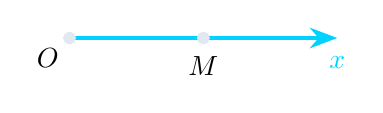
\begin{tikzpicture}[line width=1.1pt,>={Stealth[length=3.5mm]}]
  \coordinate (O) at (0,0);
  \coordinate (M) at (1.7,0);
  \coordinate (X) at (3.4,0);
  \draw[tmblue,->] (O) -- (X) node[below=3pt]{$x$};
  \tkzDrawPoints[size=3.5,color=tminc,fill=tminc](O,M)
  \tkzLabelPoint[below left](O){$O$}
  \tkzLabelPoint[below=3pt](M){$M$}
\end{tikzpicture}
\end{document}
